\documentclass{article}
\usepackage{graphicx}
\usepackage{verbatim}
\usepackage{geometry}
\usepackage{float}
\geometry{top=2cm,left=2cm,right=2cm,bottom=2cm}
\usepackage{hyperref}

\title{Milestone 2: Sketchbook}

\begin{document}

\date{}
\maketitle

\section{Project Goals}
Our main project goal is to make academic research more visible and accessible.
We begin with the field of Computer Science, but the project is designed to be scalable, with the potential to expand into other disciplines such as Physics.

A timeline visualization highlights major breakthroughs in the selected research area.
When hovering over a paper title, additional information such as a brief description becomes visible.
This concept could be further extended to highlight key developments within specific subfields.

\begin{center}
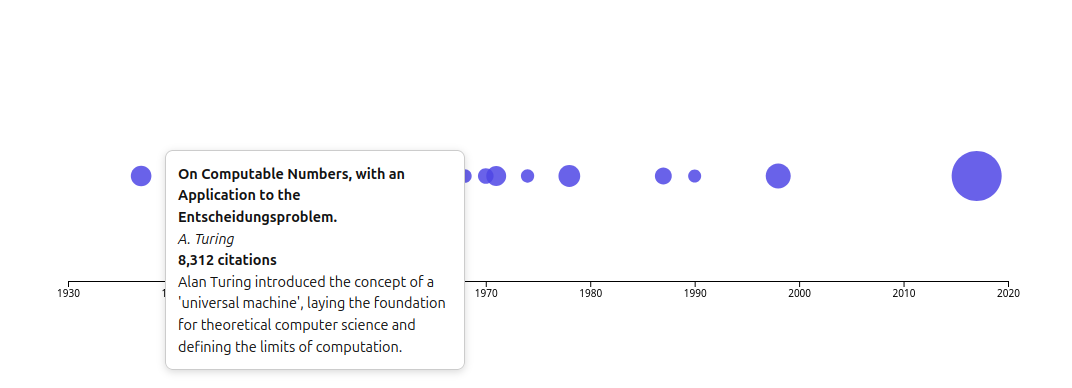
\includegraphics[width=0.6\textwidth]{./pictures/timeline.png}
\end{center}

The fields and their respective subfields (which may belong to more than one field) are represented as round buttons. These buttons become less colorful when not selected:

\begin{center}
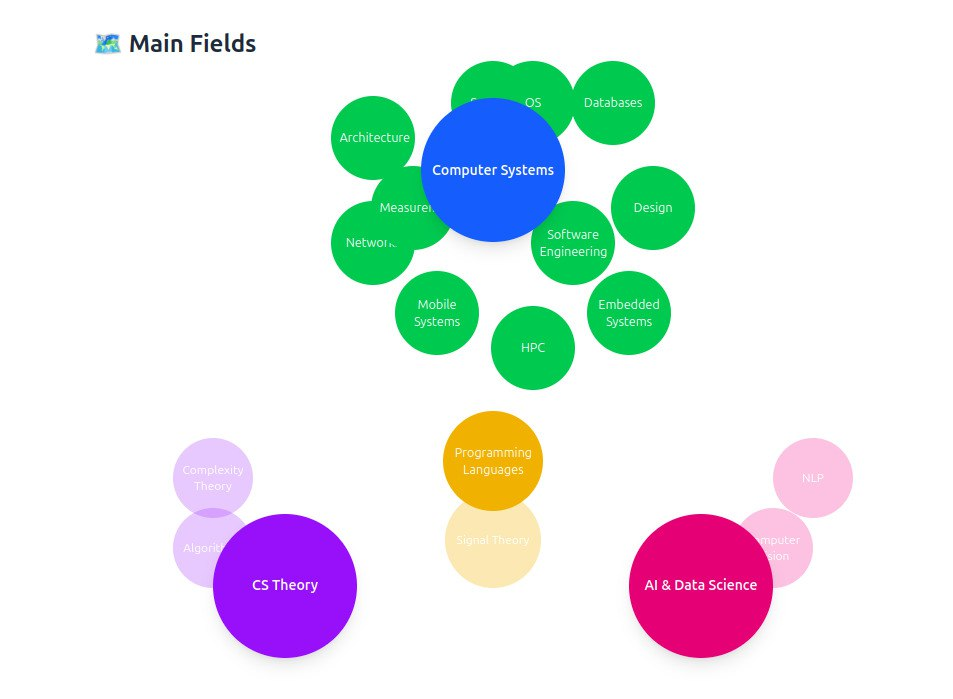
\includegraphics[width=0.6\textwidth]{./pictures/fields.jpeg}
\end{center}

We also include a list of the most cited papers and authors, with the option to filter by publication year.

\begin{center}
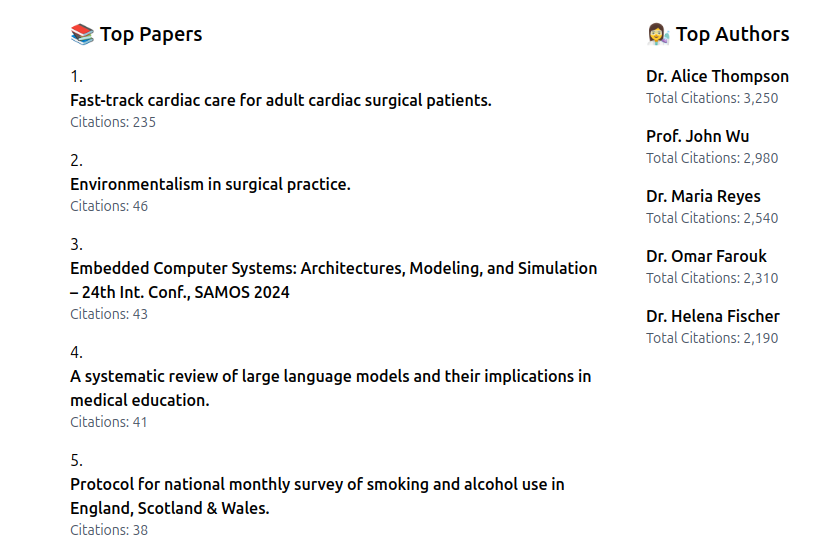
\includegraphics[width=0.6\textwidth]{./pictures/top_papers_top_authors.png}
\end{center}

A user might also be interested in identifying the most important venues.
This information can be found by examining the average citation counts,
which are visualized in a bar chart or a Sankey diagram illustrating where the most cited authors have published.
\begin{center}
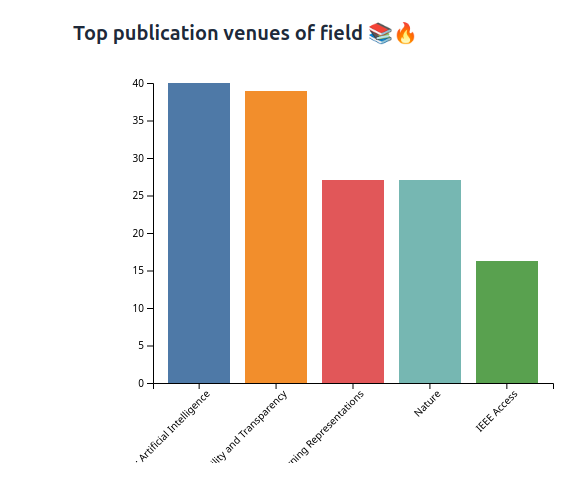
\includegraphics[width=0.6\textwidth]{./pictures/top_publication_venues.png}
\end{center}

\begin{center}
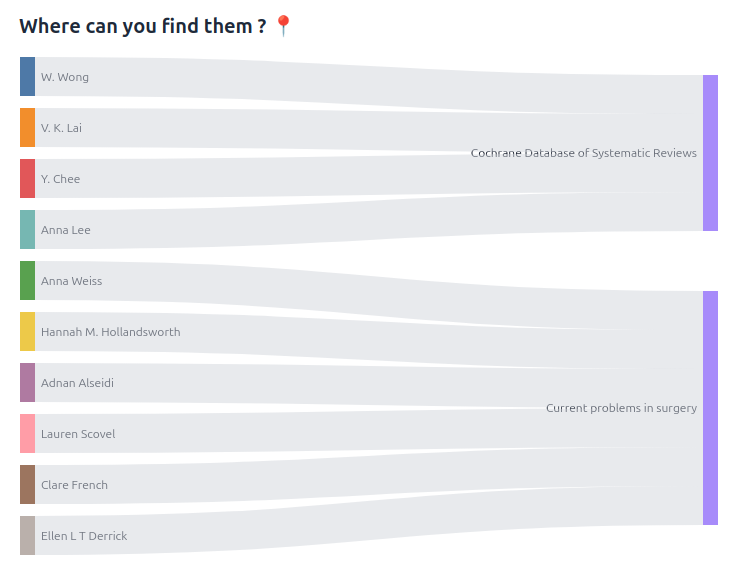
\includegraphics[width=0.6\textwidth]{./pictures/sankey.png}
\end{center}

We also plan to show the number of publications in a given field over time.
A significant increase in publications could indicate that the field has become very popular (e.g., machine learning).
Alternatively, it might suggest a decline in quality, possibly due to venues becoming less selective in accepting papers.

\begin{center}
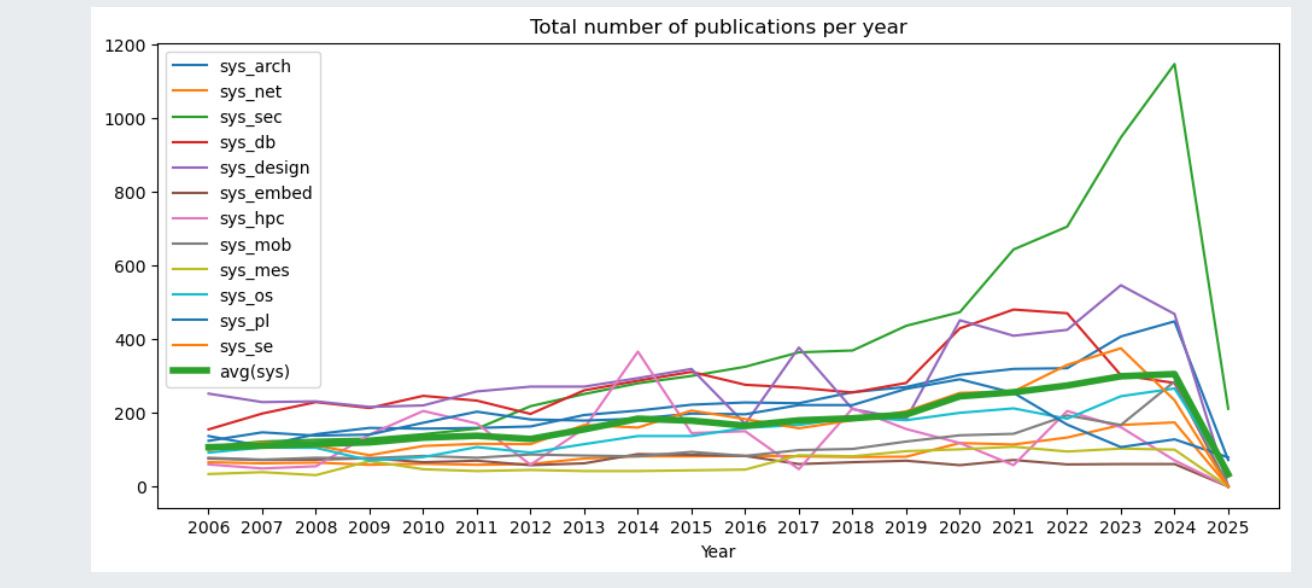
\includegraphics[width=0.8\textwidth]{./pictures/number_of_publications.png}
\end{center}

Some of these visualizations \href{https://com-480-data-visualization.github.io/DSM/}{are already live on the website}, though currently populated with dummy data for demonstration purposes.

\subsection{Additional Ideas}
As an additional idea, we could implement a connectivity graph of authors, visualizing their collaborations or citation relationships.
A similar concept has already been explored by Prof. Payer, but there’s definitely room for us to improve the styling and user experience. ;-)

\begin{center}
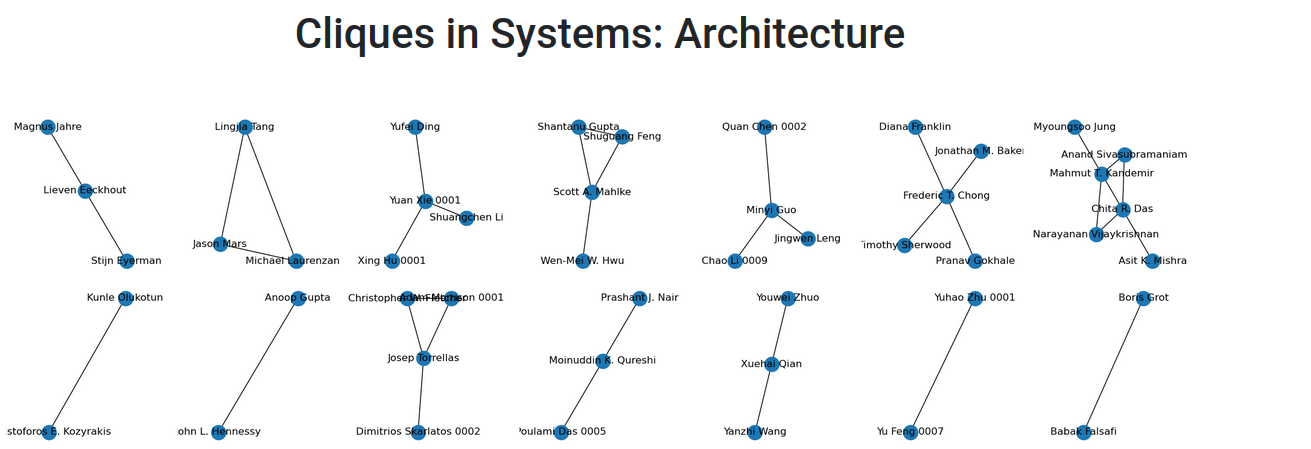
\includegraphics[width=0.9\textwidth]{./pictures/cliques.png}
\end{center}

For the most relevant papers, we could also create a graph-based interface that allows students to browse papers more intuitively, by exploring connections between them.

These two visualizations pose greater challenges—not only in terms of visual complexity, but also due to the demanding data preprocessing involved.
As such, they will require more development time and certainly more CPU cycles.

Another idea is to create an ancestral gallery showcasing all Turing Award winners.
Each laureate would be represented with a portrait, and when hovering over a photo, a short summary of their contribution would appear.
Clicking the image could take users to the official ACM Turing Award page for more in-depth information.

\begin{center}
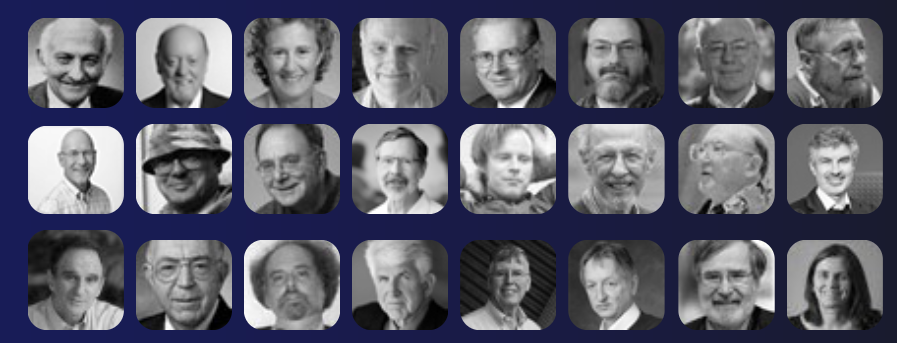
\includegraphics[width=0.9\textwidth]{./pictures/ancestor_galery.png}
\end{center}

\section{Tools and Technologies Used for Visualizations}
For our visualizations, we will use the D3.js library to create dynamic, interactive data graphics.
To simplify styling and layout, we will use Tailwind CSS instead of plain CSS.

We have already set up the project repository with Node.js, which gives us a development environment with features such as live reloading.

To maintain consistent code style, we use Prettier for code formatting.
Linting rules are enforced via our GitHub CI pipeline, which also handles automatic deployment of commits to the main branch directly to the website hosted on GitHub Pages.

\section{Relevant Lectures}
Dos and Donts cover important general advice we will try to follow.
The lectures about D3.js and interactions with D3.js as well as their exercises are helpful in using the chosen library.
To show the relationsships between authors or to have citation graphs the future lectures about graphs could be useful.

\end{document}
